\chapter{Minimum-Violation Planning for Urban Air Mobility}%\blfootnote{The chapter material is published in~\cite{bharNFMminviol}. Tichakorn Wongpirormsarn provided technical insight into minimum violation planning. Joey Muffoletto helped in implementing the experiments. Natasha Neogi provided datasets for simulation as well as subject matter expertise from NASA.}
In general, it is not always feasible to guarantee the satisfaction of all safety constraints under all conditions. Such scenarios are explicitly accounted for in 14 CFR \S 107.21, which allows for emergency deviation from regulations if required as long as the deviation is reported. For example, a vehicle may have to make an emergency landing if it is about to run out of fuel, even if violates separation requirements. Thus, there is a need for an air traffic management approach that allows for \emph{formally justifiable} violation of safety constraints if necessary. The following presents our work on the synthesis of control strategies for automated air traffic management for UAM while obeying safety regulations. In particular, we focus on the case where all safety regulations cannot be feasibly satisfied, which is allowed for small, cargo-carrying UAS under emergency operation. We present a decentralized, scalable synthesis approach that provably \emph{minimally violates} the given safety requirements.  Note that if it is possible to satisfy all safety properties for the duration of the flight, the approach yields a solution with zero violations (i.e., all safety requirements are guaranteed for the duration of the flight). 

Our approach is based on minimum-violation planning for systems that are subject to potentially infeasible safety requirements. Given a prioritized safety specification, which specifies the priority and weight of each safety requirement, minimum-violation planning computes a plan that minimally violates the requirements. In particular, we propose a novel \emph{decentralized approach} to minimum-violation planning in order to handle large-scale systems that cannot be handled by current state-of-the-art approaches. 

%\section{Minimum violation planning}

\subsection{Problem significance}
Recent years have seen increased urbanization, economic expansion, underinvestment in infrastructure, and the rise of ride hailing services and e-commerce.  These changes have led to an increase in transportation delays, vehicle congestion during peak times, and environmental impacts resulting in escalating mobility challenges in urban areas. The emerging Urban Air Mobility (UAM) aviation market is being catalyzed by advances in increasingly autonomous systems, electric propulsion, and novel business models such as on-demand, aerial ride sharing, thereby helping to address congestion issues in urban areas~\cite{flightplan2030}.  

UAM has the potential to be a safe, functional solution to the air transportation problem for passengers and cargo in and around a densely populated urban area.  An air traffic management system that governs a large number of these novel UAM operations over a small geographical area in a safe and efficient fashion is key to the realization and deployment of the UAM vision.  The notion of on-demand, (near) point-to-point mobility that transits people or goods over congested urban areas offers the potential for reduced transit times, as well as decreased environmental impact, for low-noise, electrified UAM vehicles.  Note that due to the near point-to-point nature of the solution, UAM operations must be tightly integrated with local communities and existing modes of transportation. 


\subsection{Scalable and Verifiable Safety for UAM}
The scale and density of projected UAM operations will far exceed the safe workload capacity of human controllers, necessitating the deployment of increasingly autonomous solutions for functions like aircraft management (e.g., managing flightpath and altitude requests, managing airborne and ground based holding times, etc.) and aircraft separation.

Currently, there is no established infrastructure for air traffic management of a scalable UAM concept of operations. Under current aviation paradigms, air traffic management is carried out in a centralized fashion by air traffic controllers.  The U.S. National Airspace System (NAS) is comprised of 5.3 million square miles of domestic airspace and 24 million square miles of oceanic airspace.  There are approximately 5,000 flights airborne at any given moment.  Over 14,000 air traffic controllers manage these aircraft and perform multiple safety-critical functions, such as air traffic separation which guarantees that a minimum spacing between aircraft is maintained \cite{FAAData}.  In contrast, for UAM operations to deploy at scale for profit, it will be necessary to have hundreds (or even thousands) of UAM aircraft aloft over an urban airspace under 500 square miles~\cite{goyal2018urban}.  The sheer number of vehicles, along with the necessary reduced separation criteria between them in order to achieve the required densities, will require the development of increasingly autonomous capabilities for aircraft clearance, separation, and flow management in the UAM ecosystem.  

Deploying increasingly autonomous systems in the US airspace is a challenge. Commercial aviation is among one of the most safety-critical systems in the world and has stringent standards for the design, deployment, and operation of aircraft and air traffic control systems. These regulations are detailed in chapter 14 of the Code of Federal Regulations (14 CFR). The ability to assure increasingly autonomous systems to aviation grade standards is thus crucial for their acceptance.  Safety-critical functions such as aircraft separation must provide strict guarantees on their behavior and the correctness of their outcomes.  Thus, increasingly autonomous air traffic management systems will have to tackle the dual issues of scalability and verifiable safety in order to be deployed in the NAS.


\subsection{Setting}
 In this paper, we employ a hierarchical decomposition of the UAM operations space motivated by the physical and geographical infrastructure required to field the system. Such an architecture has been studied in~\cite{bhnfm,bhTCNS} and allows for scalable air traffic management.  UAM vehicles take off and land from a landing pad, called a vertipad, which includes the final approach and takeoff (FATO) area.  A vertiport is comprised of several vertipads, the respective vertipad FATOs, and charging and maintenance facilities.  A vertihub is comprised of several vertiports.  Vertihubs provide air traffic control services (i.e., real time control of aircraft movement) between vertiports under their control and air traffic management services (i.e., strategic and long term planning of aircraft movement and flows) for vehicles transiting between adjacent vertihubs.  Figure~\ref{fig:uam_architecture} provides a visual representation of vertiports and vertihubs.  We focus on a synthesis strategy for vertihubs, each of which is responsible for assuring the safety of all vehicles in its airspace.  


\begin{figure}
    \centering
    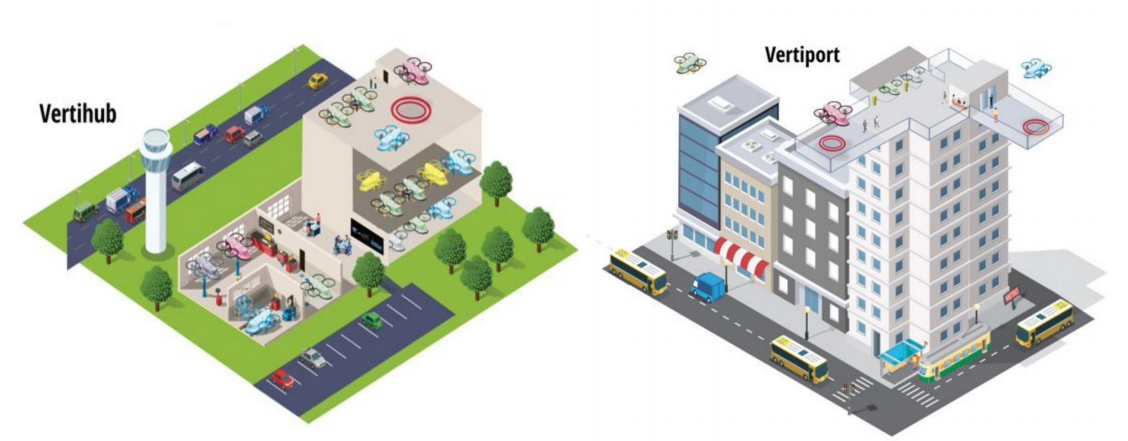
\includegraphics[width=0.98\columnwidth]{UAM-NFM/Figures/vert.PNG}
    \caption{Vertihub and vertiport depiction}
     \label{fig:uam_architecture}
\end{figure}

In general, it is not always feasible to guarantee the satisfaction of all safety constraints under all conditions. Such scenarios are explicitly accounted for in 14 CFR \S 107.21, which allows for emergency deviation from regulations if required as long as the deviation is reported. For example, a vehicle may have to make an emergency landing if it is about to run out of fuel, even if violates separation requirements. Thus, there is a need for an air traffic management approach that allows for \emph{formally justifiable} violation of safety constraints if necessary. In this paper, we study the synthesis of control strategies for automated air traffic management for UAM while obeying safety regulations. In particular, we focus on the case where all safety regulations cannot be feasibly satisfied, as is allowed for small, cargo-carrying UAS under emergency operation. We present a decentralized, scalable synthesis approach that provably \emph{minimally violates} the given safety requirements.  Note that if it is possible to satisfy all safety properties for the duration of the flight, the approach yields a solution with zero violations (i.e., all safety requirements are guaranteed for the duration of the flight). %\nok{I'm not sure where this would be an appropriate place to add but we should explicitly mention that in the case where all the requirements can be satisfied, our solution will indeed result in 0 violation. (There was the time when I gave a talk about minimum violation planning and a question like this came up, so it might not be obvious to everyone that by minimizing violation, we'll have 0 violation if all requirements can be satisfied.)}

\subsection{Contribution and Innovation}

We present the first decentralized approach to minimum violation planning. We use temporal logic for a formal representation of safety regulations and guarantee that these regulations are minimally violated across the global system. Furthermore, we establish a \emph{framework} in this paper for minimum-violation for the small UAS cargo-carrying application over urban areas. Our framework has the following properties:

\begin{itemize}
    \item \emph{Scalability} - UAM operations are envisioned to occur at a scale well beyond the capabilities of current air traffic management approaches, as current day approaches are typically labor-intensive. It is crucial to safely guarantee operations of increasingly autonomous vehicles at scale in order for UAM to be commercially viable. 
    
    \item \emph{Decentralization} - The environment is likely to encompass multiple service providers and stakeholders. Each stakeholder will have potentially competing priorities and requirements. Consequently, the full state of the entire system is unlikely to be controlled or even observed by a single entity.
    
    \item \emph{Transparency} - With companies ranging from startups to corporations developing UAM vehicles, services, and capabilities, there is a disconnect between regulation and the pace of technological development. Bridging the gap between regulation and real-world implementation practices is necessary for a viable path to deployment. 
    
    \item \emph{Flexibility} - The technological and regulatory landscape of UAM is rapidly changing. Any proposed framework that cannot efficiently incorporate a change in regulation or emerging capabilities is not a viable solution. 
    
    \item \emph{Auditability} - All violations of regulations must be formally accounted for and reported. Our proposed method implicitly allows for such an analysis, as it not only synthesizes a control strategy for air traffic management but also the associated violation. 
    
    % allows for \textit{a posteriori} analysis on runs of the system \nok{I'm not sure how to put this more accurately but we should mention that the framework implicitly incorporates analysis in that it does not only generate a plan but also the violation associated with the plan, so separate analysis does not need to be performed.} in order to identify and isolate the underlying cause of any decisions made by the system during execution. Hence, adjustments can be made to factors that are found to cause poor performance for the global system. \textcolor{magenta}{This one is a little tricky, for if you can predict these violations a priori, the requirement would be that you fix them.}
    \end{itemize}


\subsection{Path to deployment}

Assessing the safety of an increasingly autonomous system relies on being able to bound the behavior and interactions of the components of the system as well as its interfaces with its operational environment. Performance-based regulation is employed in aviation to specify explicit properties that must be evinced by a component or element of the system (and/or operational environment) in order for the system safety claims to be met.  For example, 14 CFR \S 107.49 (d) states that: “If the small unmanned aircraft is powered, ensure that there is enough available power for the small unmanned aircraft system to operate for the intended operational time”.  This fuel requirement forms a temporal logic constraint on the vehicle during its flight. The controller synthesis method for the vertihubs must adhere to this constraint, in order to demonstrate compliance to 14 CFR \S 107.49.  The minimum violation guarantees provided by the presented synthesis process help to demonstrate that this regulation will be satisfied as much as possible throughout the flight process.  Thus, the guarantees provided by the synthesis method presented in this paper may serve as a partial means of compliance to the regulation---supplemented with the generation of test and design analysis artifacts as well as operational procedures.

The presented synthesis framework provides a path to deployment of these increasingly autonomous systems in safety-critical contexts.  Air traffic management services, such as aircraft separation, may then be offered in a UAS Traffic Management (UTM) inspired framework, which interfaces with today’s traditional Air Traffic Management framework~\cite{PRKRJJ2016}. In this framework,  authority may be delegated by the FAA to provide select air traffic management services such as low-altitude weather information, congestion management, terrain avoidance, route planning, re-rerouting, separation management, and contingency management~\cite{MBYDLGMC2018,NCDDASC2018}.  One of the main attributes of the UTM system is that it does not require human operators to monitor every vehicle continuously, as in the traditional ATM system, thereby enabling increasingly autonomous realizations of specified air traffic management functions.  %NASA has led UTM research over the past five years, and is currently involved in the development and testing of a prototype UTM system with the FAA, in conjunction with numerous industry and public agency partners.  
We believe that integration of the approach in this paper into a UTM-like construct provides a path to deployment for UAM operations, as the provided safety guarantees will greatly enhance the assurance case for higher-risk operations currently not supported by UTM (e.g., operations in dense urban environments with UAS exceeding 55 lbs).


\subsection{Related work}
Some preliminary work is being done in cooperative ATM for next generation air traffic management \cite{prevot2005co}, but this work considers a scheduled approach for large passenger aircraft and cannot handle management for on-demand flights. Similarly, there is work done on distributed control for ATM of small unmanned aerial systems (UAS) \cite{FSLLK2015}, but this work relies on cloud based architectures that do not currently satisfy strict aviation safety requirements.  Hybrid control approaches have been applied \cite{tomlin1996hybrid}, however scalability proves to be an issue.
To the best of our knowledge, this is the first approach implementing minimally violating
controller synthesis for large-scale UAM ATM operations. Formally verified tools such as DAIDALUS~\cite{Daidalus} provide safety guarantees at lower levels of operations, however, it does not handle the fleet-level operations. Another approach called \emph{runtime enforcement}~\cite{Falcone10,Schneider00} aims to guarantee a specified property by detecting and altering the behavior of the system at runtime. An existing approach called shielding~\cite{BloemKKW15,KonighoferABHKT17} uses reactive synthesis and assumes that the shield has full knowledge and control of the whole system --- in this case the entire UAM system and the vehicles it handles. A technique for synthesizing quantitative shields for multi-agent systems in a fully centralized manner was presented in \cite{multiagentshield}. However, all these approaches are only applicable if a feasible solution exists. If it is not possible to satisfy all safety requirements, no solution is possible. In contrast, in the approach presented in this work, if no feasible solution exists, we can still synthesize a controller that minimally violates safety. 

Our approach is based on minimum-violation planning for systems that are subject to potentially infeasible safety requirements. Given a prioritized safety specification, which specifies the priority and weight of each safety requirement, minimum-violation planning computes a plan that minimally violates the requirements. In particular, we propose a novel \emph{decentralized approach} to minimum-violation planning in order to handle large-scale systems that cannot be handled by current state-of-the-art approaches. 

%
\subsection{Notation and Setting}\label{sec:background}
In this section, we present the relevant technical notation for the minimum violation synthesis problem in the UAM setting. 

%
\newcommand{\OperatorSpace}[5]{
				%\draw[rounded corners = 15pt,dashed] (#1-#4,#2-#5) rectangle (#1+#4,#2+#5);
		\fill[fill=green,opacity=0.2] (#1,#2) circle (#3);
		\draw[draw = black,dashed](#1,#2) circle (#3);
		%\node at (#1,#2-#5+0.5) {$V_{#6}$};
	}

	

		\subfloat[ Example UAM operating environment \label{fig:RegionsOutline}]{
		\scalebox{1.75}{
		\begin{tikzpicture}[scale=0.3]
			\OperatorSpace{0}{0}{3}{5}{5}
			%\node at (-4.25,4.25){$S_1$};
			\node at (-1.5,1.5){$V_1$};
			\OperatorSpace{3}{-4}{3}{5}{5}
			%\node at (-1.25,-8.25){$S_2$};
			\node at (2.5,-4.5){$V_2$};
			\node[red] at (2.5,3) (H13) {$H_{13}$};
			\draw [->,red,line width = 0.75mm] (H13) -- (2.5,1.25);
			\OperatorSpace{5}{0}{3}{5}{6}
			%\node at (5-4.25,5.5){$S_3$};
			\node at (5-0.5,2){$V_3$};
			\node[red] at (6.5,3.5) (H35) {$H_{35}$};
			\draw [->,red,line width = 0.75mm] (H35) -- (6.75,0.65);
			\OperatorSpace{10}{0}{4}{6}{7}
			
			\node at (8.5-0.5,-5.5){$V_4$};
% 			\node[red] at (6.5,3.5) (H35) {$H_{35}$};
			\draw [->,red,line width = 0.75mm] (H35) -- (6.75,0.65);
			\OperatorSpace{6.5}{-4}{2.5}{0}{0}
			
			%\node at (10+5.25,-6.5){$S_5$};
			\node at (10+1.5,-1.5){$V_5$};
			\OperatorSpace{15}{2}{3}{5}{5}
			\fill[blue] (-1.5,-1.5) rectangle (-1,-1);
			%\node at (15-4.25,5+3.25){$S_6$};
			\node at (15,3.5){$V_6$};
			\node[red] at (11,4.5) (H56) {$H_{56}$};
			\draw [->,red,line width = 0.75mm] (H56) -- (12.5,2.75);
			\draw (17,3) node[cross,blue]{};
			\draw[blue,line width = 0.5mm] plot [smooth,tension=1] coordinates{(-1.5,-1.5) (3,0.5) (10,0) (17,3)};
			\draw (-0.5,2) node[cross,black]{};
			\fill[black] (7.5,-5.5) rectangle (7.0,-5.0);
			\draw[black,line width = 0.5mm] plot [smooth,tension=1] coordinates{(-0.5,2) (3,-0.5) (7,-5.0)};
			
		\end{tikzpicture}}}\\
\subfloat[Connectivity graph \label{fig:Environment_directed}]{
\scalebox{1.25}{
\begin{tikzpicture}[auto,node distance=8mm,>=latex,font=\small]
        \tikzstyle{round} = [thick,draw=black,circle]
\tikzstyle{action} = [circle, draw, fill=black,inner sep=0pt, minimum size=4pt]
\node[round] (s1) {$\design_{1}$};
\node[round, right=15mm of s1] (s3){$\design_{3}$};
\node[round, below right=15mm and 5mm of s1] (s2){$\design_{2}$};
\node[round, right=15mm of s3] (s5){$\design_{5}$};
\node[round, right=10mm of s2] (s4){$\design_{4}$};
\node[round, right= 10mm of s5] (s6){$\design_{6}$};

\draw[<->] (s1) -- node[left]{$e_{12}$} (s2);
\path[<->,draw] (s1) -- node{$e_{13}$} (s3);
\path[<->,draw] (s2) -- node{$e_{23}$} (s3);
\path[<->,draw] (s2) -- node{$e_{24}$} (s4);
\path[<->,draw] (s3) -- node{$e_{34}$} (s4);
\path[<->,draw] (s3) -- node{$e_{35}$} (s5);
\path[<->,draw] (s4) -- node[right]{$e_{45}$} (s5);
\path[<->,draw] (s5) -- node[below]{$e_{56}$} (s6);

% \path[->,draw] (s1) edge[loop above] node {$e_{1}$} (s1);
% \path[->,draw] (s2) edge[loop below] node {$e_{2}$} (s2);
% \path[->,draw] (s3) edge[loop above] node {$e_{3}$} (s3);
% \path[->,draw] (s4) edge[loop below] node {$e_{4}$} (s4);
% \path[->,draw] (s5) edge[loop above] node {$e_{5}$} (s5);
% \path[->,draw] (s6) edge[loop above] node {$e_{6}$} (s6);

\end{tikzpicture}}}


\subsubsection{Requests}
We define a request as a tuple $ O = \left(r,T,c \right)$ where
\begin{itemize}
    \item $r \in \mathcal{R}$ is the request class from a predefined set of classes $
    \mathcal{R}$. Request classes include \emph{landing at a particular vertiport in the region}, \emph{pass-through region}, \emph{take-off from vertiport in the region}. Depending on the nature of the problem, $\mathcal{R}$ can be defined to capture all types of desired outcomes for vehicles.   
    \item $T \in \mathbb{N}$ is the amount of time left before the request \emph{must} be granted. $t$ can function as an analogue for fuel reserves as vehicles requesting to land cannot hover indefinitely. 
    \item $c \in C$ is the class of UAM vehicle from a predefined set of vehicles $C$.  
\end{itemize}
At any given timestep $t$ the vertihub is managing requests from multiple vehicles.  We define the initial set of requests as the \emph{request allocation} and denote it as $\mathcal{O}^{\text{init}}$. We model the \emph{vertihub controller} that is responsible for managing these requests as a 
\emph{labeled weighted finite transition system}. 
\begin{eg}
Tower $\mathcal{T}_1$ is given a set of $N$ requests to handle $\mathcal{O}^{\text{init}} = \{O^{\mathcal{T}_1}_1 \dots O^{\mathcal{T}_1}_N \}$. For example, $O^{\mathcal{T}_1}_1 = \left(port\, A, 5, passenger \right)$ corresponds to a request by a \emph{passenger vehicle} trying to land at port A in \emph{at most} 5 time steps. 
\end{eg}




\subsubsection{Transition system model for vertihub controller}
Recall that in the previous section, I defined the vertihub and vertiport controller models as \emph{reactive systems}. However, in the case of minimum-violation planning, we focus purely on correctness with respect to finite-time linear temporal logic specifications. As such, the current methodology cannot yet handle the full expressiveness of the reactive system definition. For the purposes of the minimum-violation planning approach we henceforth model a vertihub controller is modeled as a tuple referred to as a labeled weighted finite transition system $\mathcal{T}_i = \left(S_i, s_{\text{init}_i},\Delta_i, \text{AP}_i,L_i \right)$ where

\begin{itemize}
    \item $S_i$ is a finite state space.  It is the set of all currently unapproved requests. Formally, if there are currently $m$ unapproved requests, we write $S_i = \{O_{i,1} \dots O_{i,m}\}$. We note that the state space can also include additional features of interest such as number of vehicles in the airspace, their landing/take-off statuses, and others. However, for notational simplicity we do not include these in the definition presented in this paper. In practice, these features, alongside the relevant modifications to the transition function, are straightforward to include. 
    \item $s_{\text{init}_i} \in S_i$ is the initial set of requests $\mathcal{O}^{\text{init}}_i$.
    \item $\Delta_i \subseteq S_i \times S_i$ is the deterministic transition function that governs how requests evolve. We have $\left(S^t_i,S^{t+1}_i \right) \in \Delta_i$ if:

    \begin{itemize}
        \item all \emph{approved} requests at timestep $t$, denoted $\mathcal O_{i,a}^t \subseteq S^t_i$,  are not present in $S^{t+1}_i$, i.e., if $O_{i,j} \in  \mathcal O_{i,a}^t$ then $O_{i,j} \notin S^{t+1}_i$, and
        \item all \emph{unapproved} requests at timestep $t$, denoted $S^{t}_i \setminus \mathcal O_{i,a}^t$, have their time remaining decremented, i.e., for all $O_{i,j} = (r,T,c)$ and $O_{i,j} \in S^{t}_i \setminus \mathcal{O}_{i,a}^t$, we will have $O_{i,j} \in S^{t+1}_i$ and $O_{i,j} = (r,\max(T-1,0),c)$. Informally, if request is not approved $\Delta_i$ decrements the remaining timer on the request by 1. 
    \end{itemize}
    \item $\text{AP}$ is a set of atomic propositions.
    \item  $L:S\rightarrow 2^{\text{AP}}$ is the labeling function.
\end{itemize}

I note that this is a much less general model than the reactive system approach. Handling the full expressiveness of reactive systems is a subject of future work in minimum-violation planning. 

At every timestep, the decision problem for the controller is to choose a set $O_{i,a}^t \subseteq S^{t}_i$ of requests to approve. The controller will also have the option to reroute the request to neighboring controllers

\begin{eg}
Consider vertihub controller $\mathcal{T}_1$ with two pending requests $O^{\mathcal{T}_1}_1 = \left(port\, A, 5, passenger \right)$ and $O^{\mathcal{T}_1}_2= \left(port\, A, 3, passenger \right)$. In this case, at time step $t$ we have $S_1^t = \{O_{1,1},O_{1,2}\}$ where $O_{1,1} = O^{\mathcal{T}_1}_1$ and $O_{1,2} = O^{\mathcal{T}_1}_2$. Let us assume at time step $t$ that the controller approves request $O_{1,2}$. We denote this as $\mathcal{O}^{t}_{1,a} = \{O_{1,2} \}$ and we will have $S^{t+1}_1 = \{O_{1,2}\}$ where $ O_{1,1} = \left(port\, A, 4, passenger \right)$. 
\end{eg}


A finite trace of $\mathcal{T}_i$ is a finite sequence of states $\tau_i = s_{i,0} s_{i,1} \ldots s_{i,n}$ such that
$s_{i,0} = s_{\textit{init}_i}$ and $(s_{i,j}, s_{i,j+1}) \in \Delta_i$, for all $j \in \mathbb{N}_{\leq n-1}$.
A finite trace $\tau = s_0 s_1 \ldots s_n$ produces a finite word $w(\tau) = L(s_0) L(s_1) \ldots L(s_n)$. For any $s \in S$, we let $\text{Traces}(\mathcal{T}, s)$ represents the set of all finite traces of $\mathcal{T}$ that ends with $s$.

The aim of the transition system $\mathcal{T}_i$ is to reach a \emph{goal state} denoted $s_{\text{final}} \in S_i$. Since the hub controller needs to eventually grant all requests, $s_{\text{final}}$ corresponds to the state with no more pending requests. Formally, we have $s_{\text{final}} = \emptyset$.  

The goal of this approach is to synthesize a trace for each vertihub such that requests are accepted in a manner that satisfies all regulations. However, if this is not possible, it must approve requests in a way that minimally violates regulations. we employ linear temporal logic due to its ability to formally express a wide array or requirements. Specifically, we employ finite linear temporal logic (FLTL) to precisely describe the safety-oriented regulations. Note this FLTL has been used in the context of autonomous driving to formally represent road safety laws for planning~\cite{Tumova:2013:ACC,Tumova:2013:LCS}. 

\subsubsection{Finite linear temporal logic}
An FLTL formula is built up from the same logical notation as the LTL formulas defined earlier. The main point of contrast is that an FLTL formula $\psi$ over a set $\text{AP}$ of atomic propositions is interpreted over a finite word
$w = l_0 l_1 \ldots l_n \in (2^{\text{AP}})^{n+1}$,
and we write $w \models \psi$ if $w$ satisfies $\psi$.
In particular, consider $p \in \text{AP}$. Then,
$w \models p$ if and only if $p \in l_0$. Also,
$w \models \square p$
if and only if $p \in l_i$ for all $i \in \{0, \ldots, n\}$. Please refer to~\cite{gunter2002temporal} for full FLTL semantics. 

\begin{eg}
 14 CFR \S 107.49 (d) requires the vehicle to have enough power for its operations and hence, a vertihub cannot force a vehicle to loiter for too long. We can capture this as a specification $\psi = \square \{\lnot fuel\_too\_low_i\} $ where $fuel\_too\_low_i$ is an atomic proposition that is true when request $O_i = (r,T,c)$ has $T = 0$.
\end{eg}



A  \emph{non-deterministic finite automaton} (NFA) is a  tuple $\mathcal A = (Q,q_{\text{init}},\Sigma,\delta,F)$ where $Q$ is a finite set of states; $q_{\text{init}} \in Q$ is the initial state; $\Sigma$ is the input alphabet; $\delta \subseteq Q \times \Sigma \times Q$ is a non-deterministic transition relation; and $F \subseteq Q$ is the set of accepting states. 

Given an input word $w = w(1),\dots,w(n)$, a \emph{run} of $\mathcal A$ is a sequence $\rho = q_0q_1,\dots,q_n$, such that $q_0 = q_{\text{init}}$, and $q_{i-1},w(i),q_i \in \delta$ for all $1 \leq i \leq n$. We say a run is \emph{accepting} if $q_n \in F$. It can be shown that for any given FLTL formula $\varphi$ over $\text{AP}$, there exists an NFA $\mathcal{A}$ with alphabet $\Sigma = 2^{\text{AP}}$ that accepts all and only words over $\text{AP}$ that satisfy $\varphi$. Automatic translation of FLTL to NFA is proposed in \cite{}.

A \emph{weighted non-deterministic finite automaton} is a tuple $\mathcal A = (Q,q_{\text{init}},\Sigma,\delta,F,W)$ where $Q$, $q_{\text{init}}$, $\Sigma$, $\delta$ and $F$ are defined as those in the NFA and $W : \delta \rightarrow \mathbb{N}^k$, where $k \in \mathbb{N}$ is a weight function.  

Consider now a run $\rho$ in automaton $\mathcal A$ over a word $w \in \Sigma^{n}$. Let $\left(c_{i,1},c_{i,2},\dots,c_{i,k}\right) = W(q_{i},w(i),q_{i+1})$ denote the weight of the transition $\delta(q_{i},w(i),q_{i+1})$ for all $i = 1,\dots,n$. The weight of the full run $\rho$ is the component-wise sum of the weights of each transition on the run. Formally, $W(\rho) = \left(C_1,\dots,C_k \right)$, where $C_i = \sum_{j=0}^n c_{i,j}$.




\subsubsection{Prioritized safety specification}
A \emph{prioritized safety specification} is a tuple
$\mathcal{P} = (\text{AP}, \Omega, \Psi, \varpi)$ where
$\text{AP}$ is a set of atomic propositions,
$\Omega$ is a set of FLTL formulas over $\text{AP}$,
$\Psi = (\Psi_1, \Psi_2, \ldots, \Psi_N)$,
$\Psi_i \subseteq \Omega$
for all $i \in \{1, \ldots, N\}$,
and
$\varpi : \Omega \to \mathbb{N}$
is the priority function that assigns the weight to each
$\psi \in \Omega$.

\begin{eg}\label{ex:prioritized safety}
 A potential prioritized safety specification $\Psi = \{\Psi_1,\Psi_2\}$ for a vertihub to satisfy is $\Psi_1 = \{\psi_{1,1}\}, \Psi_2 = \{\psi_{2,1}, \psi_{2,2}, \psi_{2,3}\}$ where %\textbf{\textcolor{blue}{Write FLTL specs for these}}
\begin{itemize}
    \item $\psi_{1,1}$ = Never allow the timer on a request to expire. 
    \item  $\psi_{2,1}$ = Do not land vehicles past a vertiport's capacity.
    \item  $\psi_{2,2}$ = Do not allow more than $M$ vehicles in the vertihub's airspace at a time.
    \item  $\psi_{2,3}$ = Do not land a vehicle at a vertiport it did not request.
\end{itemize}
\end{eg} 

Note that the requirements at level i are strictly more important than those at level i+1, i.e., the system first attempts to minimize the amount of violation of level-1 requirements. Then among all the policies that minimize the violation of level-1 requirements, it attempts to minimize the amount of violation of level-2 requirements, and so on. In Example~\ref{ex:prioritized safety}, the first specification is the highest priority and the remaining specifications are all of equal priority. We use this example in the case study detailed in the Experimental Results section.

\subsubsection{Lack of safety}
Consider an FLTL formula $\psi$ over $\text{AP}$ and a finite word $w = l_0 l_1 \ldots l_n \in (2^{\text{AP}})^{n+1}$.
The \emph{lack of safety} of $w$ with respect to $\psi$ is defined as
\begin{equation}
        \lambda(w, \psi) = \min_{I \subseteq \mathbb{N}_{\leq n} |
        \mathsf{vanish}(w, I) \models \psi}
        |I|,
\end{equation}
where for any given finite sequence $w = l_0 l_1 \ldots l_n$
and a set $I \subseteq \mathbb{N}$,
$\mathsf{vanish}(w, I)$ is defined as a subsequence of $w$ obtained by
removing all $l_i$, $i \in I$.

Let $\mathcal{P} = (\text{AP}, \Omega, \Psi, \varpi)$ be a prioritized safety specification where $\Psi = (\Psi_1, \Psi_2,$ $\ldots, \Psi_N)$.
We define the \emph{lack of safety} of $w$ with respect to $\mathcal{P}$ as
\begin{equation}
        \lambda(w, \mathcal{P}) = (\lambda(w, \Psi_1), \ldots, \lambda(w, \Psi_N))
        \in \mathbb{N}^{N},
\end{equation}
where for each $i \in \{1, \ldots, N\}$,
\begin{equation}
        \lambda(w, \Psi_i) =
        \sum_{\psi \in \Psi_i} \varpi(\psi) \lambda(w, \psi).
\end{equation}

Note that there are two mechanisms to address the unequal importance of safety specifications. Namely, the prioritization of specifications by $\Psi$ and the weighting function $\varpi(\psi)$.  The weights $\varpi$ indicates the importance among different requirements within the same level.

The lack of safety of a trace $\tau$ of a finite transition system with respect to $\mathcal{P}$
is defined based on its produced word, i.e., $\lambda(\tau, \mathcal{P}) = \lambda(w(\tau), \mathcal{P})$.
The standard lexicographical order is used to compare the lack of safety between different traces.

\paragraph{Remark}
There are two mechanisms to specify the unequal importance of different specifications, the hierarchy $(\Psi_1, \Psi_2, \ldots, \Psi_N)$ and the weights captured by $\varpi$.
As the standard lexicographical order is used to compare the lack of safety between different traces, the algorithm first minimizes the lack of safety with respect to the specifications in $\Psi_1$.
Then, among all the traces that minimizes the lack of safety with respect to $\Psi_1$, it minimizes the lack of safety with respect to the specifications in $\Psi_2$, and so on.
The weights $\varpi$ only matter for the specifications within the same level of hierarchy.
%%



\subsection{Problem Formulation}




%Note that when a vehicle makes a request $r$ from a hub controller it \emph{self-reports} the values for $t,c$. An adversarial (or selfish) agent can take advantage of such a framework. For the purposes of this paper we assume vehicles report these numbers faithfully. Alternatively, there are proposals for a centralized database that all hub controllers have access to in order to verify information from agents. \textbf{From talks with Skygrid, not sure if there is any citations for this}. 




% \subsubsection{Transition system model for vertihub controller}
% A vertihub controller is represented by a tuple $\left(\mathcal{O}^{\text{init}}_i,\mathcal T_i\right)$ where $\mathcal{O}^{\text{init}}_i$ is the request allocation for the tower $\mathcal T_i$ and $\mathcal{T}_i = \left(S_i, s_{\text{init}_i},R_i, \text{AP}_i,L_i,\mathcal W_i\right)$ is a weighted transition system where

% \begin{itemize}
%     \item $S_i$ is of the set of all currently unapproved requests. Formally, if there are currently $m$ unapproved requests, we write $S_i = \{O_{i,1} \dots O_{i,m}\}$
%     % \nok{In the previous section (in the definition of requests), request is represented by $\mathcal{O}$. Probably easier to change the notation in the definition to $\mathcal{R}$.
%     % Also, instead of using the tuple notation 
%     % $S_i = \left(\mathcal{R}_{i,1} \dots \mathcal{R}_{i,m}\right)$,
%     % we should use the set notation
%     % $S_i = \left\{\mathcal{R}_{i,1} \dots \mathcal{R}_{i,m}\right\}$,
%     % i.e., change $(\ldots)$ to $\{\ldots\}$}
%     \item $s_{\text{init}_i}$ is the initial set of requests $\mathcal{O}^{\text{init}}_i$.
%     \item $R_i$ is the transition function that governs how requests evolve. We have $\left(S^t_i,S^{t+1}_i \right) \in R_i$ if:
%     \todo{I think all the $\mathcal{R}$ in the bullets below should be $\mathcal{O}$}
%     \begin{itemize}
%         \item all \emph{approved requests} at timestep $t$, denoted $O_{i,a}^t \subseteq S^t_i$,  are not present in $S^{t+1}_i$, i.e., if $O_{i,j} \in  O_{i,a}^t$ then $\mathcal{R}_{i,j} \notin S^{t+1}_i$, and
%         \item all unapproved requests at timestep $t$, $S^{t}_i \setminus \mathcal{R}_{i,a}^t$ have their time remaining decremented, i.e., for all $\mathcal{R}_{i,j} = (D_{i,j},T_{i,j}.C_{i,j})$ and $\mathcal{R}_{i,j} \in S^{t}_i \setminus \mathcal{R}_{i,a}^t$, we will have $\mathcal{R}_{i,j} \in S^{t+1}_i$ and $\mathcal{R}_{i,j} = (D_{i,j},\max(T_{i,j}-1,0).C_{i,j})$
%     \end{itemize}
% \end{itemize}
% Informally, $R_i$ removes a request from $S_i$ if it is approved, and decrements the remaining timer on the request if it is not. At every timestep, the decision problem for the controller is to choose a set $R_{i,a}^t \subseteq S^{t}_i$ of requests to approve. 

% We note that the state space can also include additional features of interest, such as number of vehicles in the airspace, their landing/take-off statuses, and others. However, for notational simplicity we do not include these in the definition presented in this paper. In practice, these features alongside the relevant modifications to the transition function are straightforward to include. 

% The aim of the transition system is to reach a \emph{goal state} denoted as $s_{\text{final}} \in S_i$. Since the hub controller needs to eventually grant all requests, $s_{\text{final}}$ corresponds to the state with no more pending requests. Formally, we have $s_{\text{final}} = \emptyset$.  





\subsubsection{Global system}
The global system is the composition of the vertihub controllers. Assume we have $N$ vertihub controllers $\mathcal{T}_1 \dots \mathcal{T}_N$. Recall that I defined a connectivity graph $G_{\mathcal{T}}$ as a directed graph with each vertex corresponding to a controller. Two controllers are \emph{connected} if they share an edge in the connectivity graph. Let $connect(\mathcal T_i)$ be the set of hub controllers $\mathcal{T}_j$ where $i \neq j$, that share an edge with $\mathcal{T}_i$. For example, in Figure~\ref{fig:RegionsOutline}, overlapping hub regions share an edge in the corresponding directed graph in Figure~\ref{fig:Environment_directed}, and therefore the corresponding controllers are connected. 

Formally, the global system is a tuple $(\mathcal{O}^{\text{init}},\Phi, \mathcal{T})$ where $\mathcal{O}^{\text{init}} = \{O_1,\dots,O_M\}$ is the global set of requests across all vertihubs, $\Phi: \{\mathcal{T}_1, ..., \mathcal{T}_N\} \rightarrow 2^{|\mathcal{O^{\text{init}}}|}$ is the \emph{request allocation function} such that $\Phi(\mathcal{T}_i)$ is the request set allocated to hub $\mathcal{T}_i$, and $ \mathcal{T}= \left(S, s_{\text{init}},\Delta, \text{AP},L\right)$ is a networked composition of $N$ hub controllers $\mathcal{T}_1,\dots,\mathcal{T}_N$ such that:
\begin{itemize}
    \item $S = \left(S_1, S_2, \dots, S_N\right)$ where $S_i$ is the set of all currently unapproved requests assigned to hub $\mathcal{T}_i$.
    Note, however, that due to possible reallocation of requests, it is not necessary that $S_i$ only contains the requests in $s_{\text{init}_i}$. Instead, it contains requests in $\bigcup_i s_{\text{init}_i}$ such that each request is assigned to at most one hub, i.e., $S_i \cap S_j = \emptyset$ for all $i, j$.
    \item $s_{\text{init}} = \left(s_{\text{init}_1},s_{\text{init}_2},\dots,s_{\text{init}_N} \right)$
    \item $\Delta \subseteq S \times S$ such that $\left(S^t, S^{t+1}\right) \in \Delta$ if for each unapproved request $O_i = (r, T, c) \in S^t_i$ at each hub $\mathcal{T}_i$,
    \begin{itemize}
    \item it remains unapproved with its time remaining decremented and either assigned to the same hub, i.e., $O_i = (r, T-1, c) \in S^{t+1}_i$, or a connected hub, i.e., $O_i = (r, T-1, c) \in S_j^{t+1}$ for some $\mathcal{T}_j \in connect(\mathcal{T}_i)$, or
    \item it is approved by hub $\mathcal{T}_i$ or a connected hub $\mathcal{T}_j \in connect(\mathcal{T}_i)$, i.e., $O_i \in \mathcal{O}^t_{i,a} \cup \mathcal{O}^t_{j,a}$, in which case the request is not present in $\bigcup_k S_k^{t+1}$.
    \end{itemize}
    \item $ \text{AP} =  \text{AP}_1 \cup  \text{AP}_2 \cup \dots \cup  \text{AP}_N$
    \item $L : S \to 2^{\text{AP}}$ such that $L(s_1, \ldots, s_N) = \bigcup_i L_i(s_i)$.
\end{itemize}

%\begin{itemize}
%    \item $S = \left(S_1,S_2,\dots,S_N\right)$ where $S_i$ is the statespace of %the hub $\mathcal{T}_i$
%    \item $s_{\text{init}} = %\left(s_{\text{init}_1},s_{\text{init}_2},\dots,s_{\text{init}_N} \right)$
%    \item $R \subseteq S \times S$. We construct $R$ as follows
%    \begin{itemize}
%        \item  $R = \left(\tilde{R}_1, \tilde{R}_2,\dots,\tilde{R}_N\right) %\cup \left(\overline{R}_1, \overline{R}_2,\dots,\overline{R}_N\right)$ where %$R_i \subseteq S_i \times S_i $ and $\overline{R}_i = S_i \times S_j$ for all %$j \in connect(i)$.
%    \end{itemize}
%    \item $ \text{AP} =  \text{AP}_1 \cup  \text{AP}_2 \cup \dots \cup  %\text{AP}_N$
%    \item $L = (L_1,L_2,\dots, L_N)$ with $L_i = S_i \rightarrow %2^{\text{AP}_i}$
%\end{itemize}


Put simply, we construct the transition function $\Delta$ as the composition of \emph{intra-hub} transitions and \emph{inter-hub} transitions. Since vehicles can only move between neighbouring hubs, \emph{inter-hub} transitions are limited to occurring only between those hubs that are connected in the graph $G_{\mathcal{T}}$.
% Hubs have the ability to redirect air vehicles to neighbouring regions. In order to capture this ability, the global system cannot be a simple composition of the individual hub controllers. The state space of a hub controller can be affected by the actions of its neighbours. We capture this ability by modifying the transition function $R_i$ for each controller $\mathcal T_i$. We define a new transition function $\tilde{R}_i$ where given $S^t_i$, $S^{t+1}_i$ is constructed by applying the following steps:
% \nok{We probably don't need this anymore. But please check that I don't miss anything in the definition of the transition system}
% \begin{enumerate}
%     \item $S^{t+1} =  S^{t}_i \setminus \mathcal{R}_{i,a}^t $
%     \item $S^{t+i}_i = \left(S^{t+i}_i \setminus \{\bigcup_{j \in connect(\mathcal T_i)}\mathcal{R}^{j,t}_{i,b}\} \right)\bigcup_{j \in connect(\mathcal T_i)} \mathcal{R}^{j,t}_{j,b}$
% \end{enumerate}
% where $\mathcal{R}^{i,t}_{j,b}$ is the set of requests transferred from controller $\mathcal{T}_i$ to $\mathcal{T}_j$. Informally, the modified transition function allows for transition systems connected in $G_{\mathcal{T}}$ to transfer vehicles between each other. The price of decentralizing the system is the loss of the additional options captured in $\tilde{R}$.
%\textcolor{blue}{finish ex}
%\begin{example}\label{ex:reallocreq}
%Consider request $S_1^{0} = \{O^{\mathcal{T}_1}_1 = \left(port\, A, 5, passenger \right),O^{\mathcal{T}_1}_2= \left(port\, A, 3, passenger \right)\}$ corresponding to a request by a \emph{passenger vehicle} trying to land at port A in \emph{at most} 5 time steps. 
%\end{example}



\subsubsection{Vertihub violation cost}
Each vertihub $\mathcal{T}_i$ is given a prioritized safety specification $\mathcal{P}_i$ and request allocation $\Phi(\mathcal{T}_i) = s_{\text{init}_i}$. Given a request allocation function $\Phi$, the \emph{violation cost} of vertihub $\mathcal{T}_i$ executing a finite trace $\tau_i \in \text{Traces}(\mathcal{T}_i,s_{\text{final}})$ 
is denoted $\lambda_{\Phi(\mathcal{T}_i)}(\tau_i,\mathcal{P}_i)$. We denote the \emph{optimal} violation cost of $\mathcal{T}_i$ for a request allocation function $\Phi$ as $\lambda_{\Phi(\mathcal{T}_i)}^* = \min_{\tau_i \in \text{Traces}(\mathcal{T}_i,s_{\text{final}})} \lambda_{\Phi(\mathcal{T}_i)}(\tau_i,\mathcal{P}_i)$. 
%where $\tau_i^*$ is the \emph{minimally violating trace} for tower $\mathcal{T}_i$ corresponding to request allocation $\Phi(\mathcal{T}_i)$. 

The cost of the global system $\mathcal{T}$ is dependent on the conjunction of the prioritized specifications $\mathcal{P} = \mathcal{P}_1 \wedge \mathcal{P}_2 \wedge \dots \wedge \mathcal{P}_N$, global requests $\mathcal{O}^{\text{init}}$, and request allocation function $\Phi$. Formally, we define
\begin{equation}
    \lambda_{\Phi} = \sum_{i=1}^N\lambda_{\Phi(\mathcal{T}_i)}^*.
    \label{eq:global-cost}
\end{equation}



% \subsubsection{Optimal violation cost}
% Given N vertihub controllers $\mathcal{T}_1,\mathcal{T}_2,\dots,\mathcal{T}_N$, and corresponding prioritized safety specifications $\mathcal{P}_1,\dots,\mathcal{P}_N$, and request allocations $\mathcal{O}^{\text{init}}_1,\dots,\mathcal{O}^{\text{init}}_N$ we define the \emph{locally optimal} total cost as $\lambda_{l}^* = \sum_{i=1}^N \lambda_{\mathcal{O}^{\text{init}}_i}^*(\tau_i,\mathcal{P}_i)$.


% The \emph{globally optimal} total cost is defined with respect to the joint system $\mathcal{T}$, prioritized specification $\mathcal{P} = \mathcal{P}_1 \wedge \mathcal{P}_2 \wedge \dots \wedge \mathcal{P}_N$, global request allocation $\mathcal{O}^{\text{init}}$, and request allocation function $\Phi$. We define

% \begin{equation}
%     \lambda_{gl}^* = \lambda_{\mathcal{O}^{\text{init}}}(\tau^*,\mathcal{P})
% \end{equation}
% where 
% where $\tau^* \in \text{Traces}(\mathcal{T},s_{final})$ is the globally minimal violating trace. Note that in general, $\lambda_{gl}^* \leq \lambda_{l}^*$. 

% \textbf{Questions}:
% \begin{itemize}
%     \item Is it true that $\lambda_{gl}^* = \lambda_{l}^*$. If so, under what conditions?
%     \item Does $\lambda_{gl}^* = \lambda_{l}^*$ imply that $\tau^* = \left(\tau_1,\dots,\tau_N \right)$?
% \end{itemize}


% \subsubsection{Optimal request allocation}
% The optimal $\lambda^{\ast}$ as the optimal cost

\subsubsection{Minimum-violation planning problem statement} 
Given a set of $N$ hub controllers $\mathcal{T}_1 \dots \mathcal{T}_N$, a connectivity graph $G_{\mathcal{T}}$ and a prioritized safety specification for each controller $\mathcal{P}_1,\dots,\mathcal{P}_N$ with $\mathcal{P} = \mathcal{P}_1 \wedge \dots \wedge \mathcal{P}_N $, construct a request allocation function $\Phi$ and corresponding trace $\tau^* = \{\tau_1,\dots,\tau_N\}$ where  $\tau_i \in  \text{Traces}(\mathcal{T}_i,s_{\text{final}})$ that minimizes the lack of safety for the entire system. Formally,

\begin{equation}
    \tau^* = \argmin_{\tau \in \{\text{Traces}(\mathcal{T},s_{\text{final}})\}} \lambda(\tau, \mathcal{P}).
\end{equation}


\subsection{Solution Approach}

Motivated by the cost structure in (\ref{eq:global-cost}), we decompose the traffic management problem into two subproblems:
\begin{enumerate}
	\item Compute an optimal request allocation $\Phi^*$ such that
	\begin{equation*}
		\sum_{i=1}^N \lambda_{\Phi^*(\mathcal{T}_i)}^* \leq \sum_{i=1}^N \lambda_{\Phi(\mathcal{T}_i)}^*,
	\end{equation*}
	for any request allocation $\Phi$. Informally, the optimal request allocation $\Phi^{*}$ will have a lower or equal cost compared with any other allocation. 
	\item Given a request allocation $\Phi$, compute an optimal trace $\tau_i^*$ for each vertiport $\mathcal{T}_i$ such that
	\begin{equation*}
		\lambda_{\Phi(\mathcal{T}_i)}(\tau_i^*, \mathcal{P}_i) \leq \lambda_{\Phi(\mathcal{T}_i)}(\tau_i, \mathcal{P}_i),
	\end{equation*}
	for any trace $\tau_i \in \text{Traces}(\mathcal{T}_i,s_{\text{final}_i})$.
\end{enumerate}
The second problem can be solved using minimum-violation planning as in~\cite{Tumova:2013:ACC,Tumova:2013:LCS}.
To solve the first problem, we need to find the globally optimal request allocation for all the vertihubs. This is a combinatorially hard problem. To solve the problem in a distributed manner, we propose an auction-based algorithm. In each round, each vertihub identifies potential requests to be reallocated and offers each of these requests to other connected vertihubs.  The request with highest cost is then selected, and a connected vertihub accepts this request if it can accommodate the extra request with less cost than the original vertihub. Finally, the request will be reallocated to the vertihub that can accommodate the request with the lowest cost. This auction-based request allocation ensures that the overall cost decreases in each round and terminates when no more requests can be reallocated without extra cost.

\subsubsection{Algorithm} 
Given a request allocation $\Phi$, we define the cost of vertihub $\mathcal{T}_i$ accommodating a request $O$ as
\begin{equation}
	C_i^\Phi(O) = \min_{\tau_i} \lambda_{\mathcal{O}^i_O}(\tau_i, \mathcal{P}_i) - \min_{\tau_i} \lambda_{\mathcal{O}^i_{\not{O}}}(\tau_i, \mathcal{P}_i),
\end{equation}
where $\mathcal{O}^i_O = \Phi(\mathcal{T}_i) \cup \{O\}$ is the set of requests allocated to $\mathcal{T}_i$ together with the request $O$, and $\mathcal{O}^i_{\not{O}} = \Phi(\mathcal{T}_i) \setminus \{O\}$ is the set of requests allocated to $\mathcal{T}_i$ without the request $O$.

The algorithm initializes $\Phi$ based on the desired location associated with each request. Then, it updates $\Phi$ iteratively as follows.
\begin{enumerate}
	\item Initialize the set $\mathbb{O}$ of potential requests to be reallocated in this iteration as the empty set.
	\item Each vertihub $\mathcal{T}_i$ computes the cost $C_i^\Phi(O)$ for accommodating each request $O \in \Phi(\mathcal{T}_i)$. It then adds each request as well as its associated cost $(O, C_i^\Phi(O))$ to $\mathbb{O}$ for all requests $O$ with $C_i^\Phi(O) > 0$.
	\item If $\mathbb{O}$ is empty, then the algorithm terminates and outputs $\Phi$. Otherwise, we let $O^*$ be the request with the highest cost in $\mathbb{O}$ and $C^*$ be its associated cost.
	\item Each vertihub $\mathcal{T}_i$ computes the cost $C_i^\Phi(O^*)$ for accommodating $O^*$. Consider two possible cases.
	\begin{itemize}
		\item $C_i^\Phi(O^*) \geq C^*$ for all $\mathcal{T}_i$, i.e., no other vertihub can better accommodate this request. Then, the request $O^*$ is removed from $\mathbb{O}$ and the algorithm goes back to step (c) to attempt reallocating the next worst request.
		\item $C_i^\Phi(O^*) < C^*$ for some $\mathcal{T}_i$. Then, $\Phi$ is updated so that the request $O^*$ is allocated to $\mathcal{T}_{i^*}$ that minimizes the cost of accommodating $O^*$, i.e., $C_{i^*}^\Phi(O^*) \leq C_i^\Phi(O^*)$ for all $\mathcal{T}_i$. This iteration finishes and the algorithm starts the new iteration with step (a). In the case where there are multiple vertihubs with equal lowest cost $C^{\ast}$, a tie breaker heuristic, e.g., based on tower id and priority, can be used.
	\end{itemize}
\end{enumerate}

As the number of requests is finite, the cost is non-negative and strictly decreases in every iteration except the last iteration.  Thus, the algorithm is guaranteed to terminate and output a request allocation that is at least as good as the initial allocation.  This is formally stated as follows.

\begin{prop}
	Let $\Phi^{init}$ be the initial request allocation. Then, the algorithm terminates with request allocation $\Phi$ such that $\lambda_{\Phi} \leq \lambda_{\Phi^{init}}$.
	
\end{prop}

Note that for ease of presentation the algorithm assumes the vertihub network is fully connected. In implementation, it is straightforward to modify the algorithm to directly incorporate the network constraints. 

%\paragraph*{The assignment problem formulation} \suda{Not sure how we use this? Maybe in the solution section?}





%%
%\subsection{Solution Approach}

Motivated by the cost structure in (\ref{eq:global-cost}), we decompose the traffic management problem into two subproblems:
\begin{enumerate}
    \item Compute an optimal request allocation $\Phi^*$ such that
    \begin{equation*}
        \sum_{i=1}^N \lambda_{\Phi^*(\mathcal{T}_i)}^* \leq \sum_{i=1}^N \lambda_{\Phi(\mathcal{T}_i)}^*,
    \end{equation*}
    for any request allocation $\Phi$. Informally, the optimal request allocation $\Phi^{*}$ will have a lower or equal cost compared with any other allocation. 
    \item Given a request allocation $\Phi$, compute an optimal trace $\tau_i^*$ for each vertiport $\mathcal{T}_i$ such that
    \begin{equation*}
        \lambda_{\Phi(\mathcal{T}_i)}(\tau_i^*, \mathcal{P}_i) \leq \lambda_{\Phi(\mathcal{T}_i)}(\tau_i, \mathcal{P}_i),
    \end{equation*}
    for any trace $\tau_i \in \text{Traces}(\mathcal{T}_i,s_{\text{final}_i})$.
\end{enumerate}
The second problem can be solved using minimum-violation planning as in~\cite{Tumova:2013:ACC,Tumova:2013:LCS}.
To solve the first problem, we need to find the globally optimal request allocation for all the vertihubs. This is a combinatorially hard problem. To solve the problem in a distributed manner, we propose an auction-based algorithm. In each round, each vertihub identifies potential requests to be reallocated and offers each of these requests to other connected vertihubs.  The request with highest cost is then selected, and a connected vertihub accepts this request if it can accommodate the extra request with less cost than the original vertihub. Finally, the request will be reallocated to the vertihub that can accommodate the request with the lowest cost. This auction-based request allocation ensures that the overall cost decreases in each round and terminates when no more requests can be reallocated without extra cost.

\subsubsection{Algorithm} 
Given a request allocation $\Phi$, we define the cost of vertihub $\mathcal{T}_i$ accommodating a request $O$ as
\begin{equation}
    C_i^\Phi(O) = \min_{\tau_i} \lambda_{\mathcal{O}^i_O}(\tau_i, \mathcal{P}_i) - \min_{\tau_i} \lambda_{\mathcal{O}^i_{\not{O}}}(\tau_i, \mathcal{P}_i),
\end{equation}
where $\mathcal{O}^i_O = \Phi(\mathcal{T}_i) \cup \{O\}$ is the set of requests allocated to $\mathcal{T}_i$ together with the request $O$, and $\mathcal{O}^i_{\not{O}} = \Phi(\mathcal{T}_i) \setminus \{O\}$ is the set of requests allocated to $\mathcal{T}_i$ without the request $O$.

The algorithm initializes $\Phi$ based on the desired location associated with each request. Then, it updates $\Phi$ iteratively as follows.
\begin{enumerate}
    \item Initialize the set $\mathbb{O}$ of potential requests to be reallocated in this iteration as the empty set.
    \item Each vertihub $\mathcal{T}_i$ computes the cost $C_i^\Phi(O)$ for accommodating each request $O \in \Phi(\mathcal{T}_i)$. It then adds each request as well as its associated cost $(O, C_i^\Phi(O))$ to $\mathbb{O}$ for all requests $O$ with $C_i^\Phi(O) > 0$.
    \item If $\mathbb{O}$ is empty, then the algorithm terminates and outputs $\Phi$. Otherwise, we let $O^*$ be the request with the highest cost in $\mathbb{O}$ and $C^*$ be its associated cost.
    \item Each vertihub $\mathcal{T}_i$ computes the cost $C_i^\Phi(O^*)$ for accommodating $O^*$. Consider two possible cases.
    \begin{itemize}
        \item $C_i^\Phi(O^*) \geq C^*$ for all $\mathcal{T}_i$, i.e., no other vertihub can better accommodate this request. Then, the request $O^*$ is removed from $\mathbb{O}$ and the algorithm goes back to step (c) to attempt reallocating the next worst request.
        \item $C_i^\Phi(O^*) < C^*$ for some $\mathcal{T}_i$. Then, $\Phi$ is updated so that the request $O^*$ is allocated to $\mathcal{T}_{i^*}$ that minimizes the cost of accommodating $O^*$, i.e., $C_{i^*}^\Phi(O^*) \leq C_i^\Phi(O^*)$ for all $\mathcal{T}_i$. This iteration finishes and the algorithm starts the new iteration with step (a). In the case where there are multiple vertihubs with equal lowest cost $C^{\ast}$, a tie breaker heuristic, e.g., based on tower id and priority, can be used.
    \end{itemize}
\end{enumerate}

As the number of requests is finite, the cost is non-negative and strictly decreases in every iteration except the last iteration.  Thus, the algorithm is guaranteed to terminate and output a request allocation that is at least as good as the initial allocation.  This is formally stated as follows.

\begin{prop}
Let $\Phi^{init}$ be the initial request allocation. Then, the algorithm terminates with request allocation $\Phi$ such that $\lambda_{\Phi} \leq \lambda_{\Phi^{init}}$.

\end{prop}

Note that for ease of presentation the algorithm assumes the vertihub network is fully connected. In implementation, it is straightforward to modify the algorithm to directly incorporate the network constraints. 
%%
\section{Experimental results}\label{sec:UAM-NFM-experiments}
In this section, we detail the results of a case study implementing the presented algorithm\footnote{The code for the implementation can be found at \url{https://github.com/JoeMuff999/Automata-Testing}}. All experiments were run on an AMD Ryzen 5 3600x processor with 6 cores @ 4.3 Ghz and 16 GB RAM. For the purposes of this demonstration, we use the prioritized safety specifications given in Example 3. We use the toolbox \textsc{TuLiP}~\cite{wongpiromsarn2011tulip} to compute minimally violating traces. 
We randomly generate vehicle requests in a format compatible with the Mission Planner Algorithm~\cite{guerreiro2019mission} developed at NASA Langley. The data contains simulated, timestamped on-demand requests for origin-destination trips corresponding to vertiports in particular vertihubs. We then run our algorithm to minimally violate the regulations described earlier.

\subsection{Scalability}
Figure~\ref{fig:runtime} shows the runtime per iteration per vertihub for different numbers of total vertihubs as well as the number of iterations until the algorithm converges. 
\begin{figure}[h!]
    \centering
    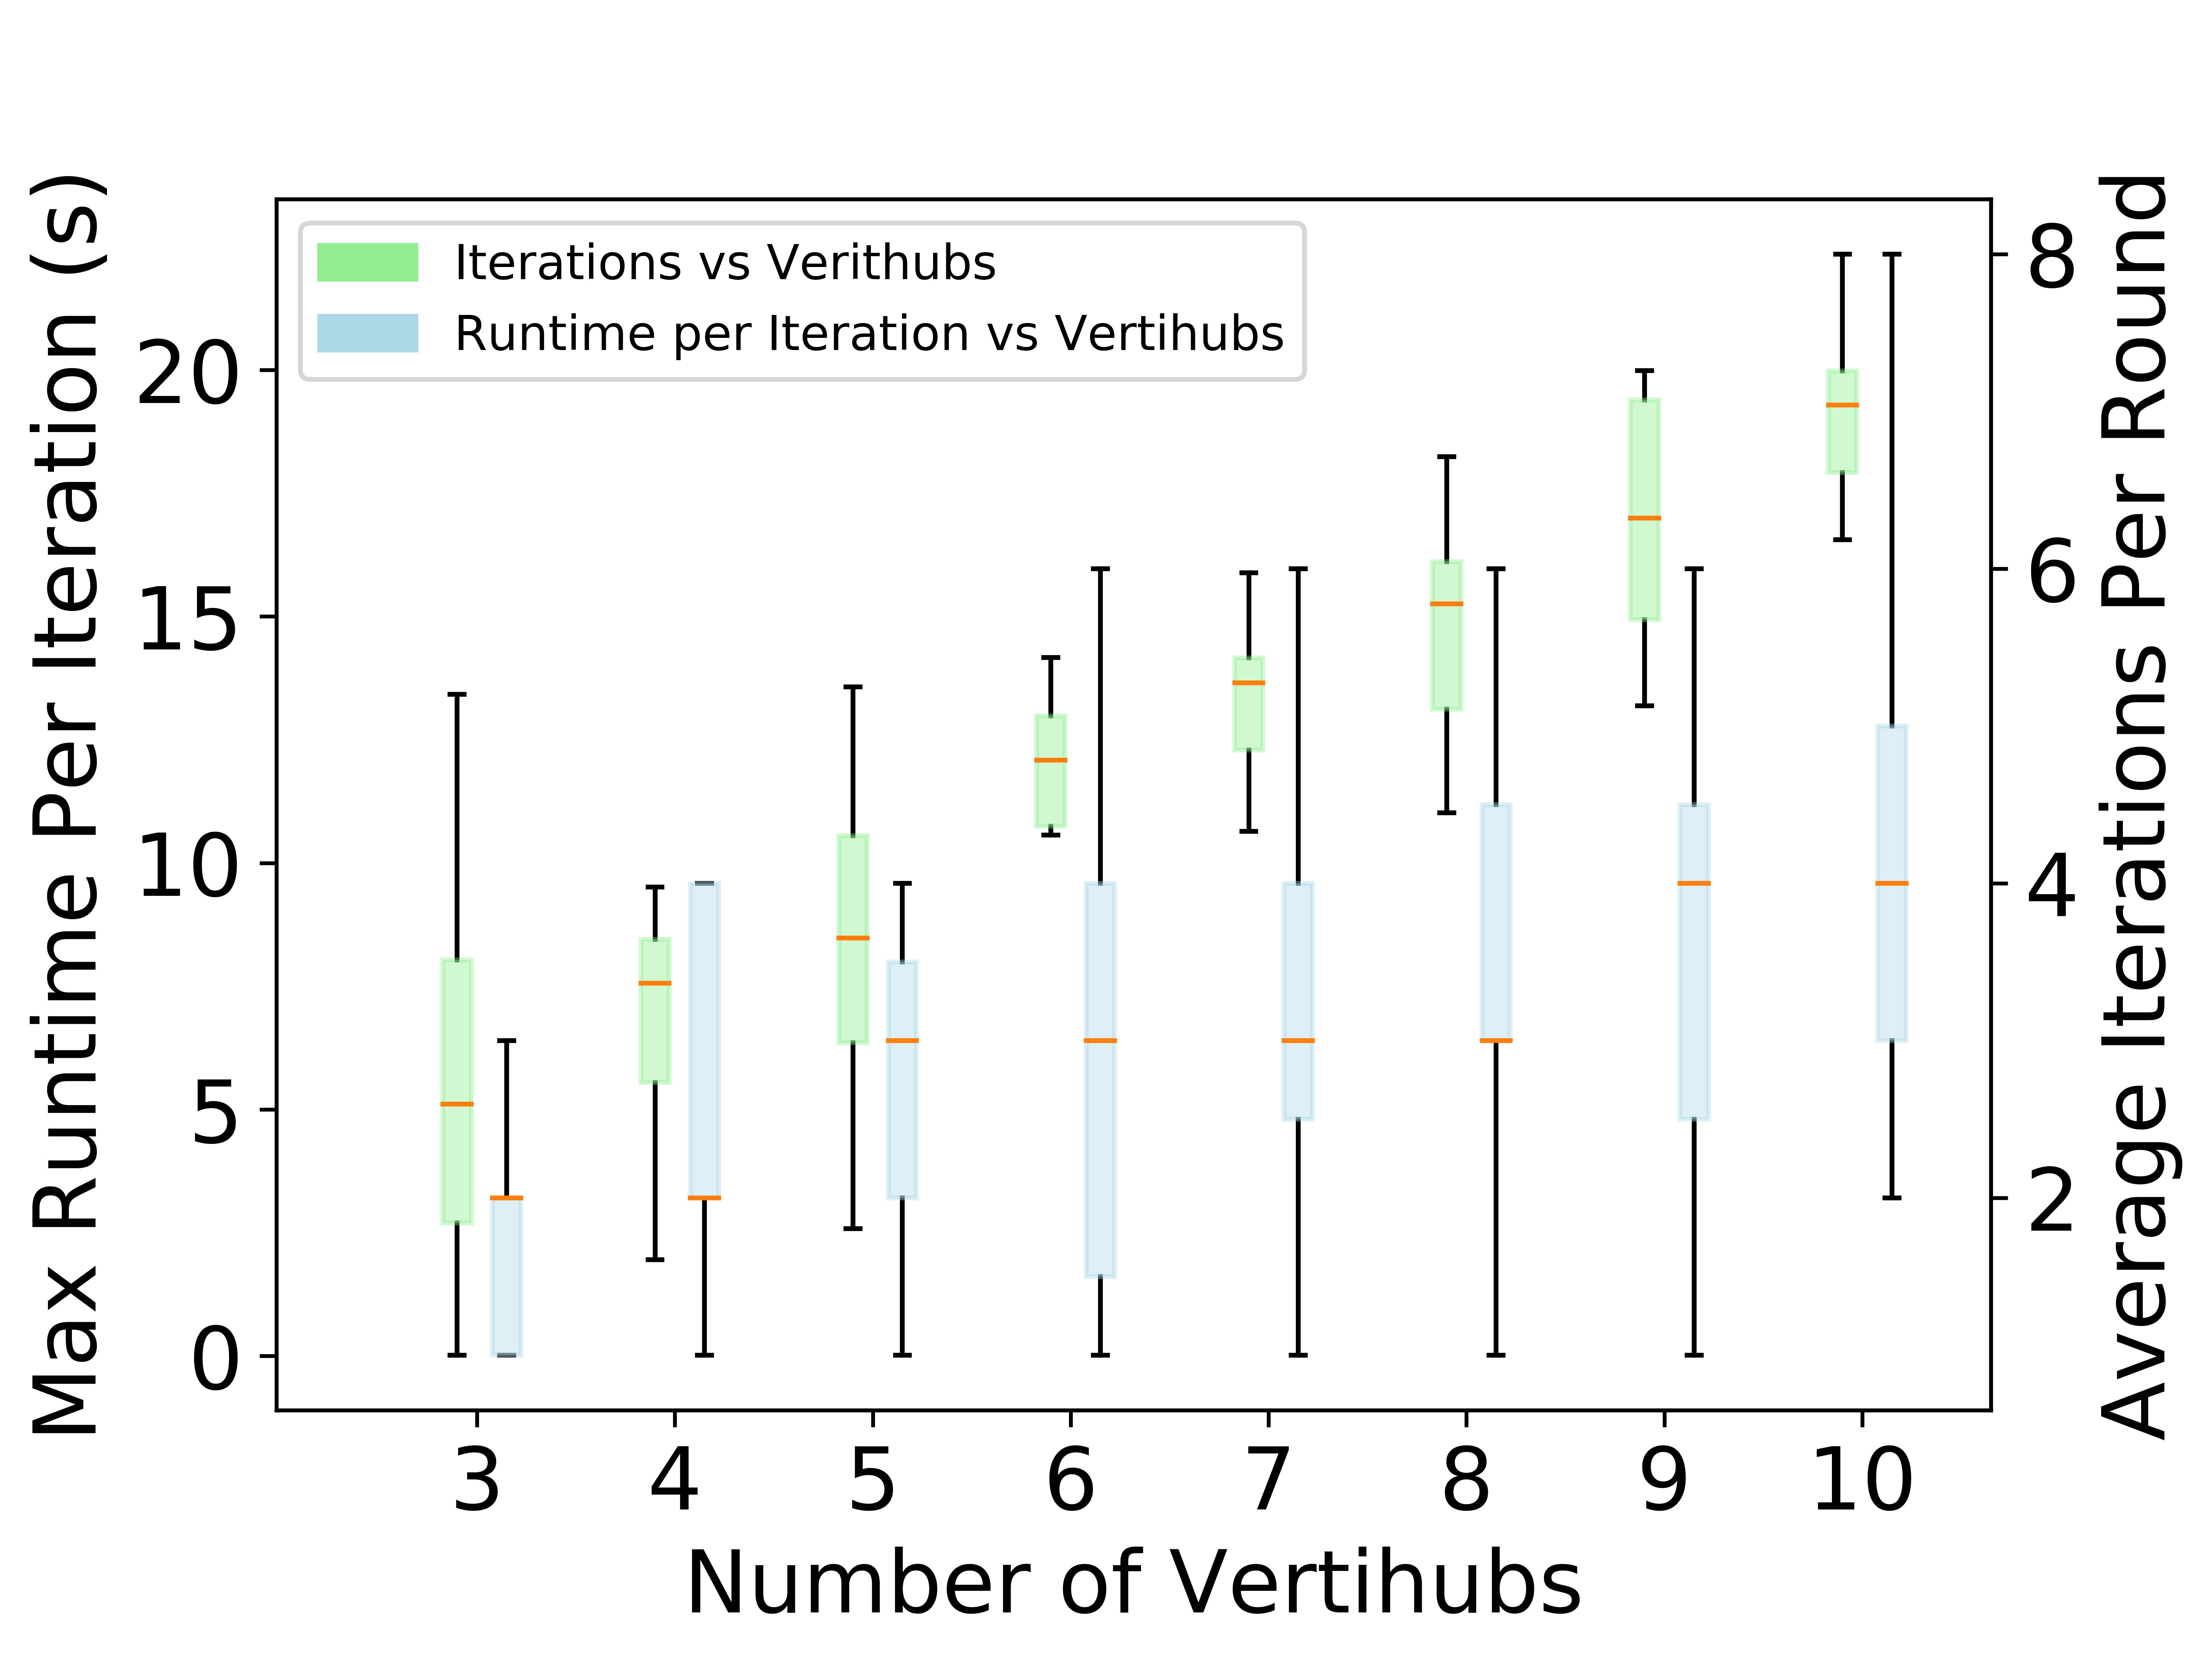
\includegraphics[width=0.8\columnwidth]{UAM-NFM/Figures/max_runtime_vs_size_boxplot_requests_static_with_iterations.png}
    \caption{Worst case runtime per iteration per vertihub (blue) and iterations until convergence (green).}
\label{fig:runtime}
\end{figure}
It is clear that the average runtime scales efficiently as the number of vertihubs increases.  In general, the total number of iterations before convergence also stays relatively constant albeit with a higher variance as the system size increases.  However, since the overall violation of the system's safety decreases with every iteration, in practice, we can always terminate the algorithm after a certain number of iterations and still have reduced the total violation cost. We note that even the smallest instance of the problem, i.e., 3 vertihubs with a maximum of 5 requests was unable to be solved in under 10 minutes using the centralized method. Furthermore, these results are a worst-case analysis as we assume the vertihubs are fully connected, i.e., all vertihubs can transfer requests to any other vertihub. In practice, the pool of vertihubs that can accept requests from other vertihubs will be smaller and this will limit the number of computations needed. 

\subsubsection{Violation cost}
To demonstrate the decreasing violation cost, we run our algorithm on the specific case of a 6 vertihub system with 10 requests. As shown in Figure~\ref{fig:costreduction}, the initial request allocation has a cost of 11 for the highest priority regulation. After 4 iterations, the cost has decreased to 0 while the cost for the second priority regulation stays at 2. 

\begin{figure}[h!]
    \centering
    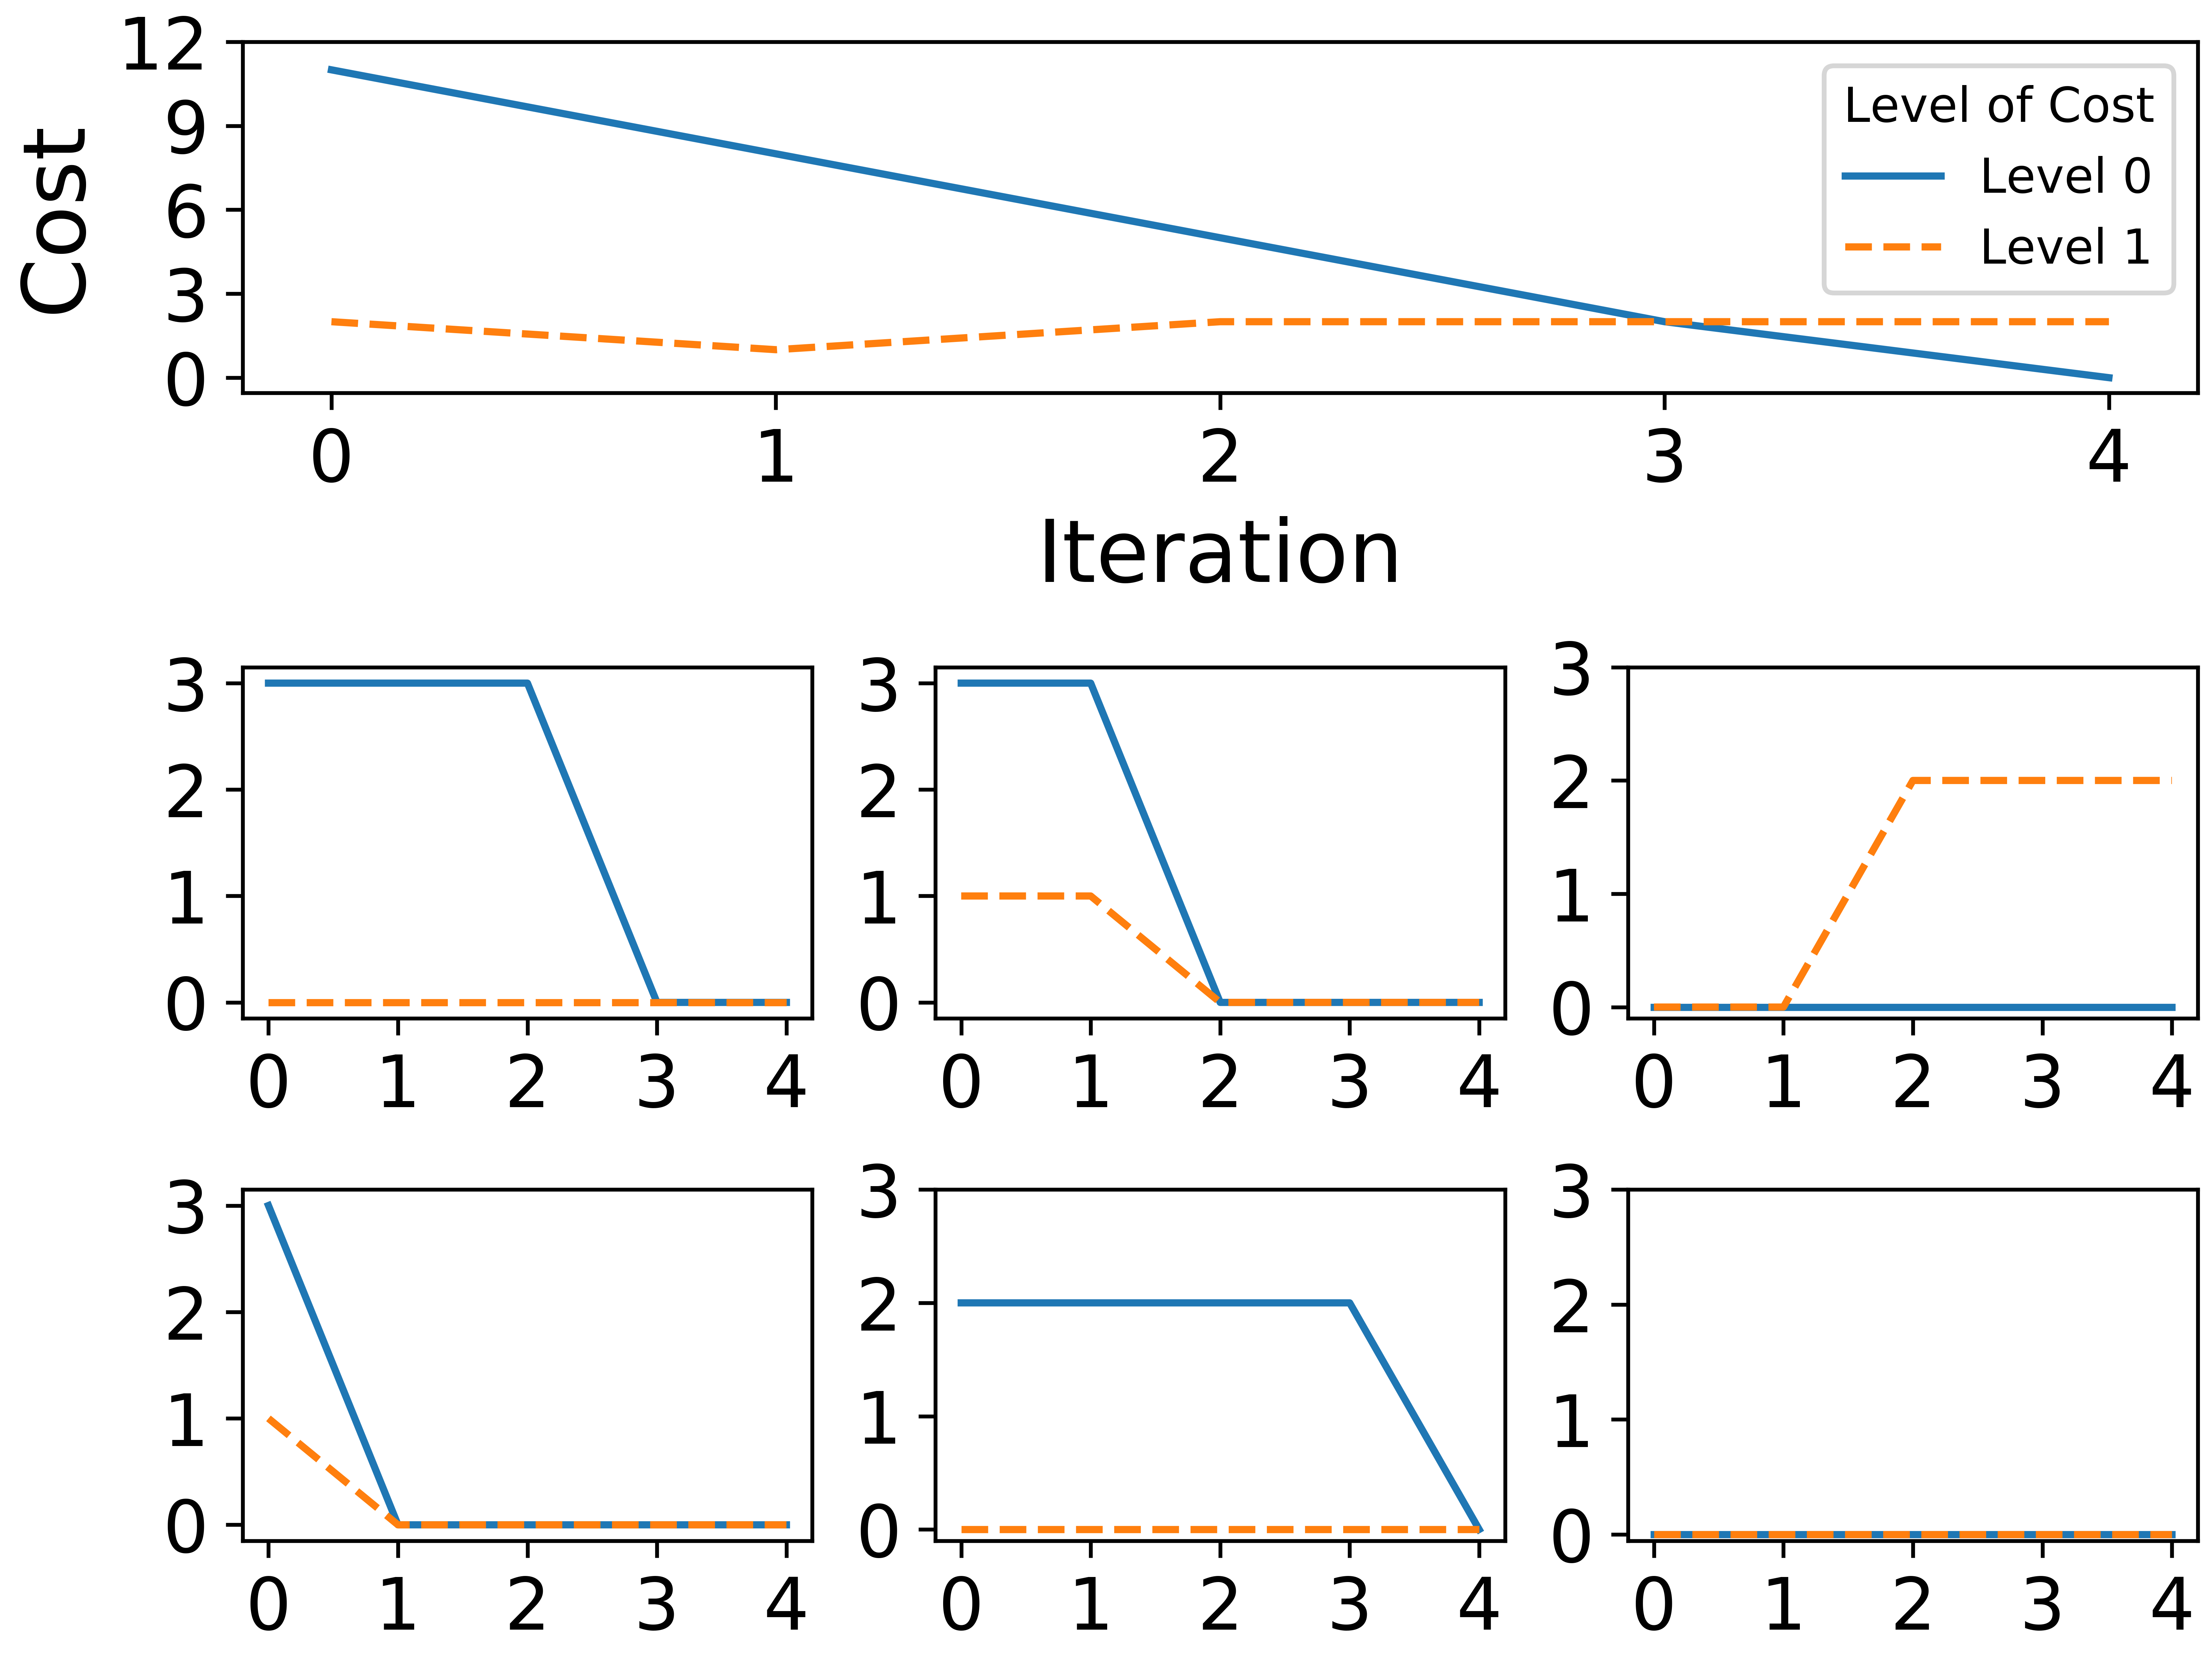
\includegraphics[width=0.85\columnwidth]{UAM-NFM/Figures/cost_vs_iteration_compiled.png}
    \caption{Violation cost vs iteration for a 6 vertihub system. Total violation, i.e., sum of the violation of all the individual vertihubs, is shown on top with the individual vertihub violation costs shown below.}
    \label{fig:costreduction}
\end{figure}



\subsection{Batch processing} The presented method in this section relies on processing batches of requests at a time. However, in practice, requests arrive sequentially in real time. In most cases however, the requests are known in advance and hence can be planned for. In this result, we demonstrate the effect of different batch sizes on overall violation cost. The data used in the simulation was generated by NASA Langley in conjunction with partners performing UAM demand studies. We divide incoming requests into batches of 5,10,and 15 requests at a time. Each batch is then processed before moving on to the next batch. We then sum the total violation cost across all batches for the entire data set. We note that we only report the level 1 violation cost as the level 0 violation cost is 0 in all cases. 

\begin{table}[]
\centering
\begin{tabular}{|c|c|c|} \toprule
Batch Size  & Violation Cost & Computation time (s) \\ \midrule
      5     &     71           &      6.6            \\
      10     &     63           &     32.5            \\
      15     &     56           &     161.9         \\ \bottomrule   
\end{tabular}
\caption{Level 1 violation cost and corresponding average synthesis time per batch per tower for different batch sizes.  } \label{tab:batchsizes}
\end{table}

As seen in Table~\ref{tab:batchsizes}, violation cost reduces as the batch size increases. This result is expected as the smaller batch sizes typically result in myopic plans that can cause violations down the road. However, it is not necessarily feasible to plan with large batch sizes as it requires a large look-ahead which may not be possible in practice. 




